\chapter{Progetto Logico}

La fase di progettazione ... avvenuta insieme al collega ... 

\section{Specifiche Funzionali}

\subsection{Autenticazione degli utenti}
Affinché un utente sia autenticato all’interno della piattaforma è necessario che esegua l’accesso tramite Google con il proprio account aziendale.

\subsection{Ruoli}
\label{ruoli}
Gli utenti che utilizzeranno le funzionalità messe a disposizione dal sistema saranno suddivisi in ruoli applicativi che individueranno chi può fare cosa all’interno del sistema. Tra i ruoli già individuati ci sono:
\begin{itemize}
    \item Membro del team
    \item Responsabile
    \item Human Resources
    \item Amministratore
    \item Data Manager
    \item Skills User
\end{itemize}
Il sistema dei permessi potrà essere successivamente esteso anche attraverso l’introduzione di nuovi ruoli, avendo cura di evitare eccessive complicazioni lato utente.

\subsection{Specifica dei Ruoli}
\subsubsection{Membro del team}
Il membro del team può:
\begin{itemize}
    \item Visualizzare i propri corsi, certificati e proposte
    \item Creare una nuova proposta con un corso da svolgere
    \item Modificare la proposta
    \item Mandare la proposta in approvazione
    \item Aggiornare lo stato di un corso in svolgimento
    \item Aggiungere un certificato già conseguito o corso già svolto in passato
    \item Assegnarsi una skill posseduta
\end{itemize}

\subsubsection{Responsabile}
Il responsabile può:
\begin{itemize}
    \item Proporre una proposta formativa ai membri del team
    \item Approvare o Rifiutare una proposta fatta da un membro del team
    \item Modificare una proposta di un membro del team e di conseguenza accettarla
    \item Visualizzare il progresso dei suoi membri del team nello svolgimento dei corsi approvati
    \item Visualizzare le competenze dei suoi membri del team
\end{itemize}

\subsubsection{Human Resources}
Tra le principali funzionalità:
\begin{itemize}
    \item Assegnare un responsabile ad un suo membro del team
    \item Aggiornare i dati relativi ad un utente
    \item Assegnare corsi e certificati già completati ai membri del team
    \item Modificare e eliminare corsi e certificati completati ai membri del team
    \item Generare report e registri per audit e conformità ISO
    \item Esportare dati relativi agli utenti
    \item Aggiornamento di utenti in blocco tramite import
\end{itemize}

\subsubsection{Data Manager}
\begin{itemize}
    \item Creare un Corso non ancora presente nel database
    \item Creare un Certificato non ancora presente nel database
    \item Creare una Categoria non ancora presente nel database
    \item Modificare e eliminare corsi, categorie, certificati e skills.
    \item Generare report e registri per audit e conformità ISO
    \item Esportare dati relativi agli utenti
    \item Aggiornamento di utenti in blocco tramite import
\end{itemize}

% Esempi di categorie: DEVOPS, SVILUPPO, FRONTEND, BACKEND, ARCHITETTURA DI SISTEMA, ANALISI.
% Esempi di Skill: Java 1/2/3, 1: Provato - 2: Usato - 3: Pro

\subsubsection{Skills User}
\begin{itemize}
    \item Utilizzare la skill matrix per cercare utenti con specifiche skills
\end{itemize}

\subsubsection{Amministratore}
Oltre ad aver accesso a tutte le funzionalità:
\begin{itemize}
    \item Esportare il database
    \item Eliminare utenti
    \item Inserimento e aggiornamento del database di più risorse contemporaneamente tramite l'upload di file csv/tsv.
\end{itemize}



\section{Requisiti funzionali del sistema}
Inviare avvisi tramite e-mail per notificare scadenze, corsi proposti, modificati e approvati al diretto interessato e al suo superiore e mostrarle nella sezione notifiche di ogni utente.

\section{Casi d’uso}
Il seguente diagramma dei casi d’uso illustra graficamente come ogni Ruolo interagisce con il sistema. Gli attori previsti nei casi d’uso sono quelli già introdotti nella sezione \ref{ruoli}, più Utente, che rappresenta l’utente generico:
\begin{itemize}
    \item Utente
    \item Membro del team
    \item Responsabile
    \item HR (Human Resource)
    \item Data Manager
    \item Skills User
    \item Amministratore
\end{itemize}


\begin{figure}[ht!]  
    \centering
            \makebox[\textwidth][c]{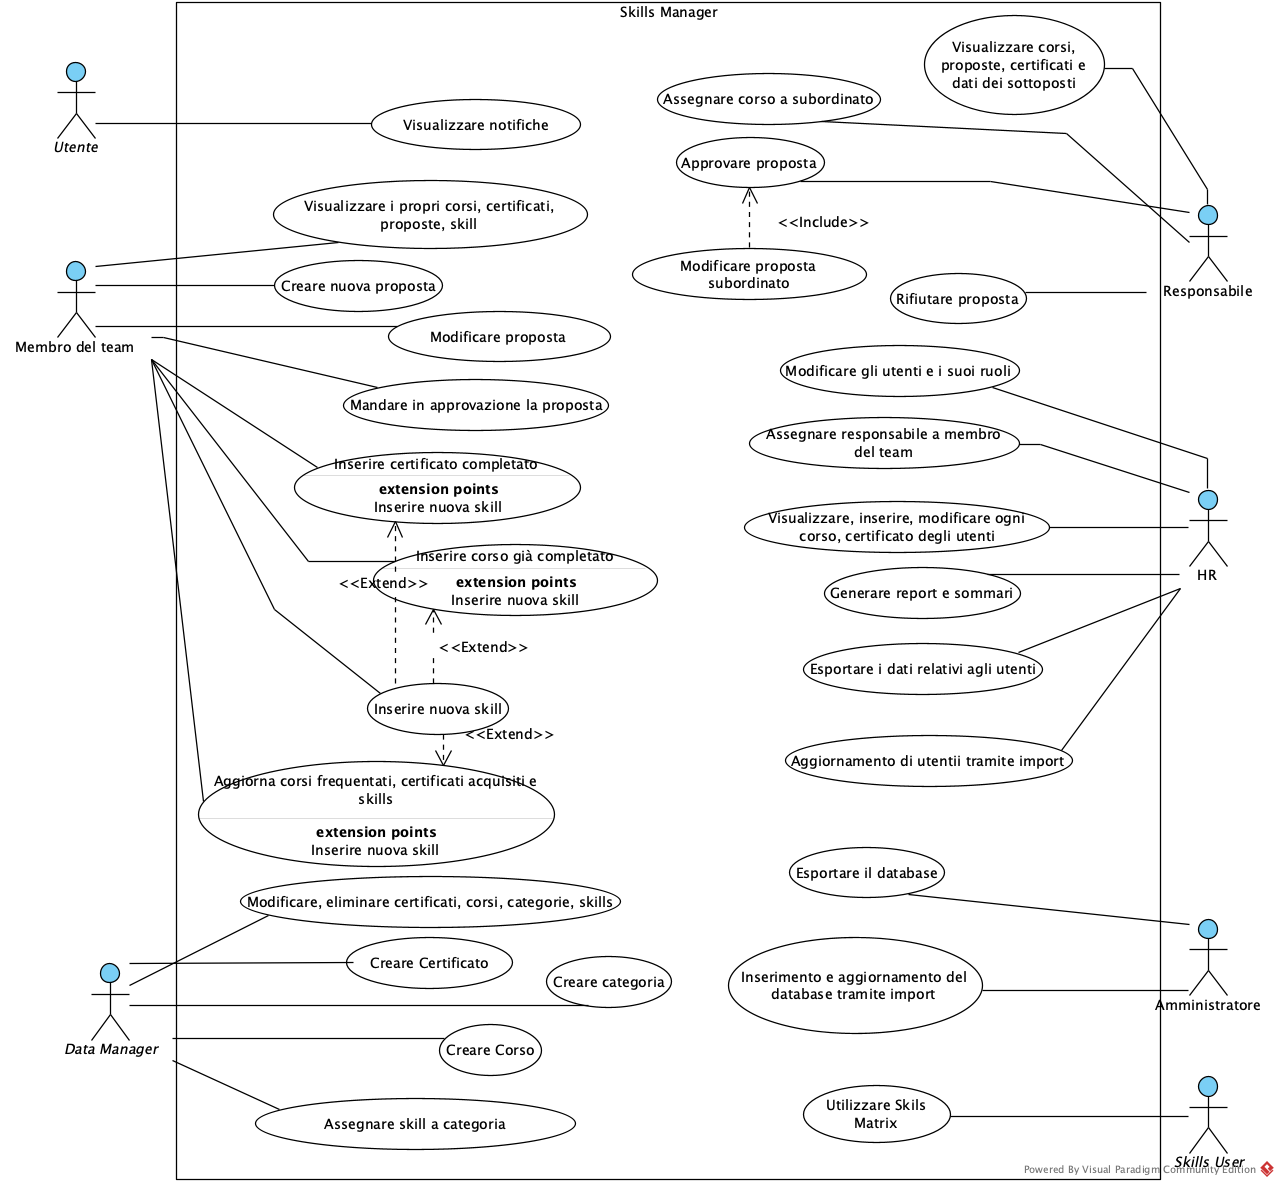
\includegraphics[width=1.2\linewidth]{immagini/casi_d'uso.png}}
        % 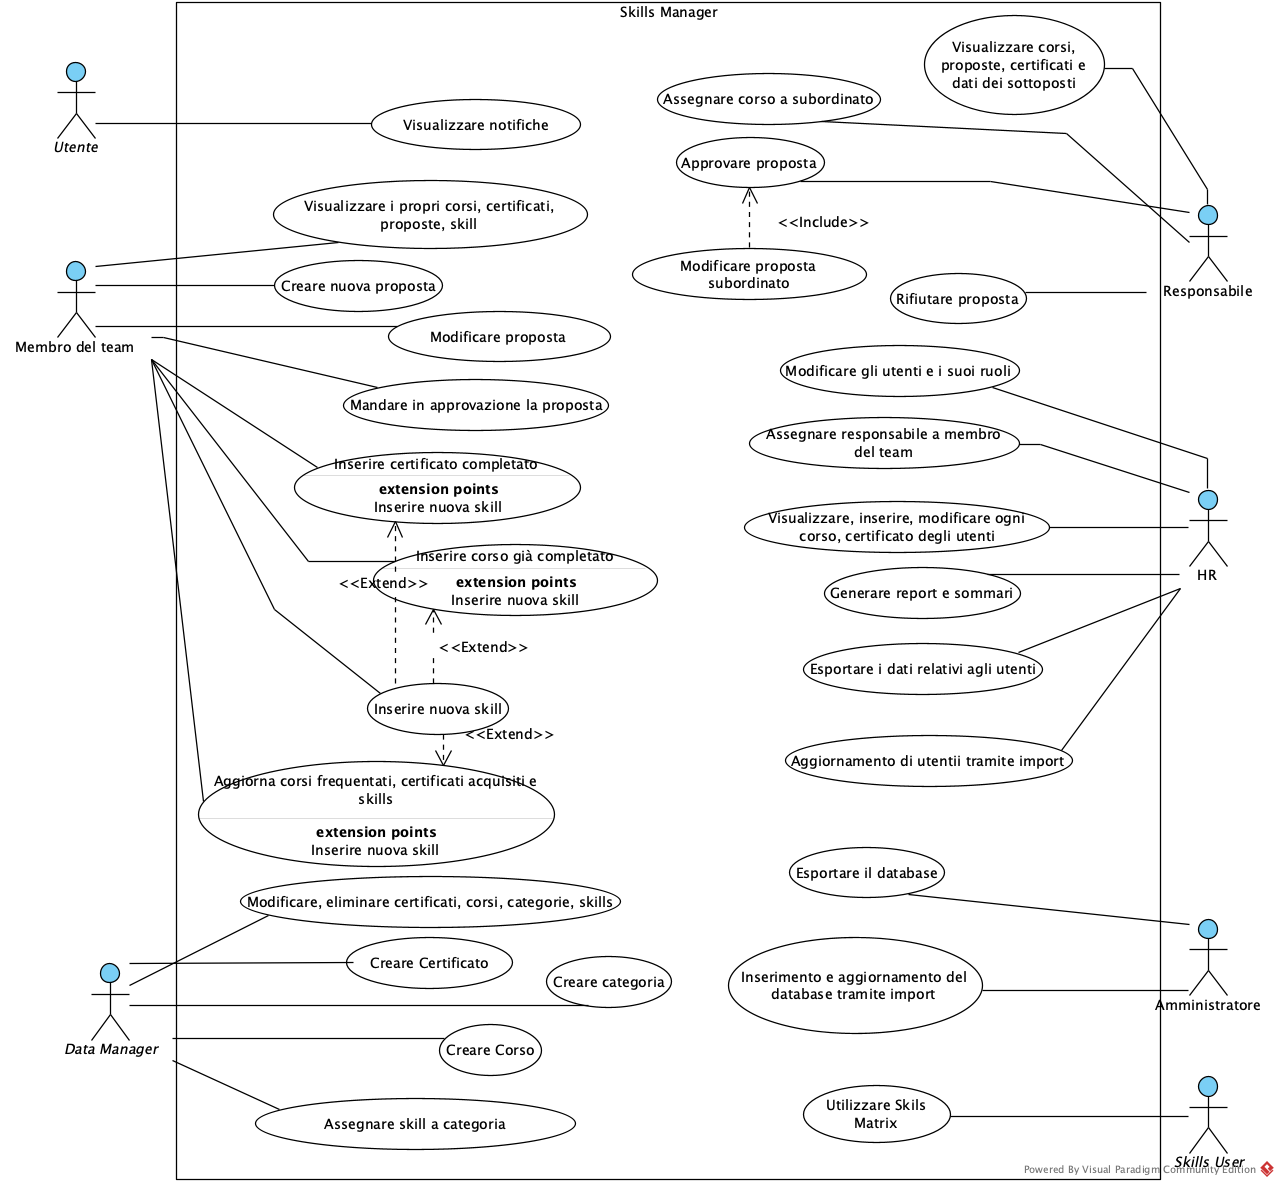
\includegraphics[width=1\linewidth]{immagini/casi_d'uso.png}
        \caption{Diagramma dei casi d'uso}
        \label{casi-d'uso} % \ref{casi-d'uso }
\end{figure}

\section{Interfaccia Grafica e Mockup}
Ogni utente ha accesso a una propria dashboard, che è composta dalle interfacce relative ai ruoli assunti all'interno del sistema. A sinistra della dashboard, gli utenti troveranno un menù contenente varie voci. Le voci del menù sono abilitate o limitate in base ai ruoli assunti dall'utente, garantendo un'esperienza personalizzata e mirata alle proprie responsabilità e competenze all'interno dell'organizzazione. Di seguito, mostro i mockup organizzati per ruolo, che illustrano le interfacce specifiche disponibili per ciascun utente in base al proprio ruolo all'interno del sistema.

\subsubsection{Membro del team}
I membri del team hanno accesso a 3 funzionalità divise in 3 pagine e voci nel menù:  
\begin{itemize}
    \item visualizzazione e aggiunta dei propri corsi in svolgimento e proposte
    \item visualizzazione e aggiunta dei propri certificati
    \item visualizzazione e aggiunta delle proprie skills 
\end{itemize}
Al momento del completamento di un corso oppure al conseguimento di un certificato sarà chiesto all’utente di aggiornare le proprie skills, che inserirà, secondo autovalutazione, quelle che ha acquisito.


\begin{figure}[ht!]  
    \centering
    \begin{minipage}{0.49\textwidth}
        \centering
        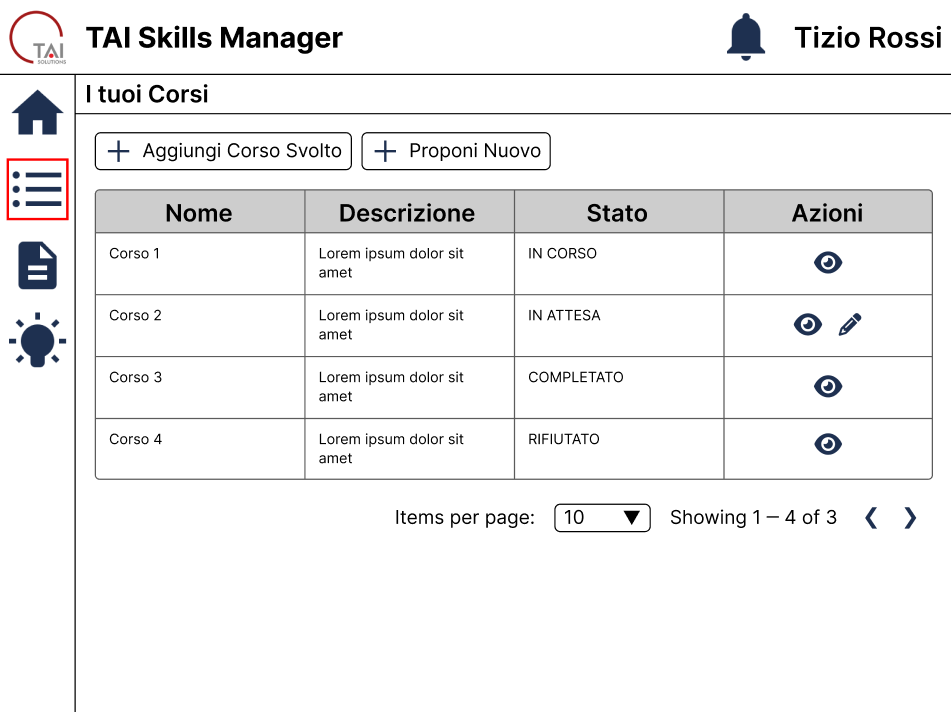
\includegraphics[width=\linewidth]{immagini/mockup/Pagina Corsi Membro del Team.png}
        \caption{Mockup della pagina Corsi di un Membro del Team}
        \label{mockup-corsi}
    \end{minipage}\hfill
    \begin{minipage}{0.49\textwidth}
        \centering
        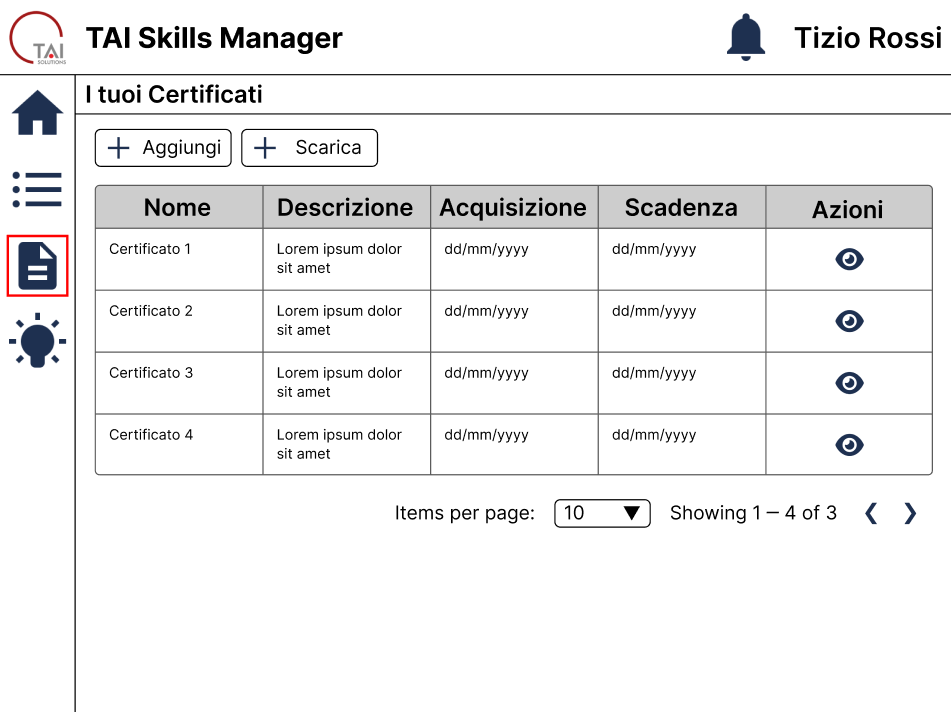
\includegraphics[width=\linewidth]{immagini/mockup/Pagina Certificati Membro del Team.png}
        \caption{Mockup della pagina Certificati di un Membro del Team}
        \label{mockup-certificati}
    \end{minipage}
\end{figure}
\FloatBarrier
\begin{figure}[ht!]  
    \centering
    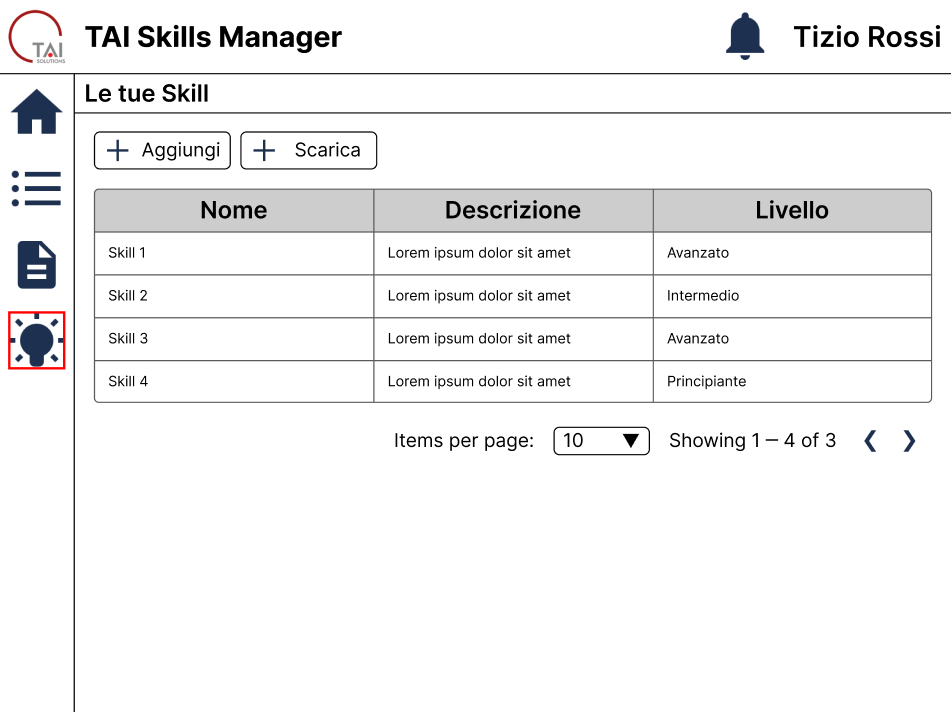
\includegraphics[width=0.49\linewidth]{immagini/mockup/Pagina Skill Membro del Team.png}
    \caption{Mockup della pagina Skills di un Membro del Team}
    \label{mockup-skills}
\end{figure}
\FloatBarrier

\subsubsection{Responsabile}
I responsabili hanno accesso alla pagina per gestire i propri membri del team, nella quale è possibile ricercare e visualizzare i dati anagrafici, corsi, e certificati di una risorsa specifica, e proporre o modificare corsi.

\begin{figure}[ht!]  
    \centering
        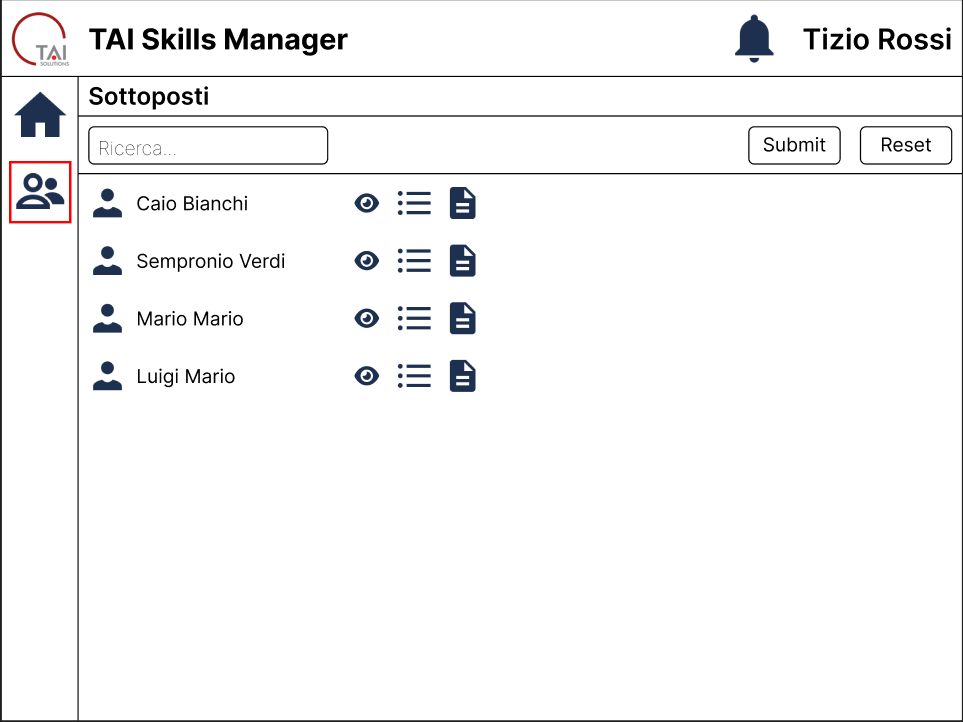
\includegraphics[width=0.7\linewidth]{immagini/mockup/Pagina Sottoposti Manager.png}
        \caption{Mockup della pagina Team di un Responsabile}
        \label{mockup-team}
\end{figure}
\FloatBarrier

\subsubsection{Human Resources}
Agli HR è fornita una pagina di browser utenti, in cui aggiornare dati anagrafici degli utenti, inserire corsi e certificati già completati ad un utente e assegnare un responsabile ad un membro del team. Inoltre in questa sezione è possibile scaricare il database degli utenti tramite file CSV, modificarlo in locale e caricarlo per fare aggiornamenti agli utenti in blocco.

\begin{figure}[ht!]  
    \centering
        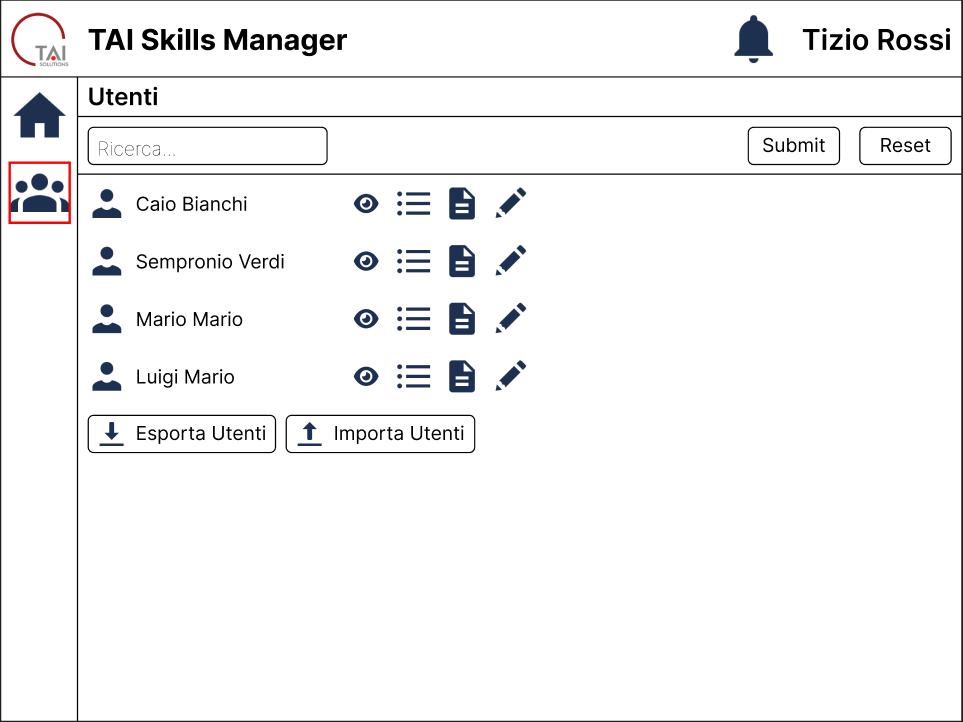
\includegraphics[width=0.7\linewidth]{immagini/mockup/Pagina Utenti HR.png}
        \caption{Mockup della pagina Utenti di un Human Resources}
        \label{mockup-utenti}
\end{figure}
\FloatBarrier

\subsubsection{Data Manager}
Nella pagina Gestione Risorse, l’utente può aggiungere al sistema certificati, corsi, skill e categorie. Inoltre può assegnare skill a categorie.

\begin{figure}[ht!]  
    \centering
        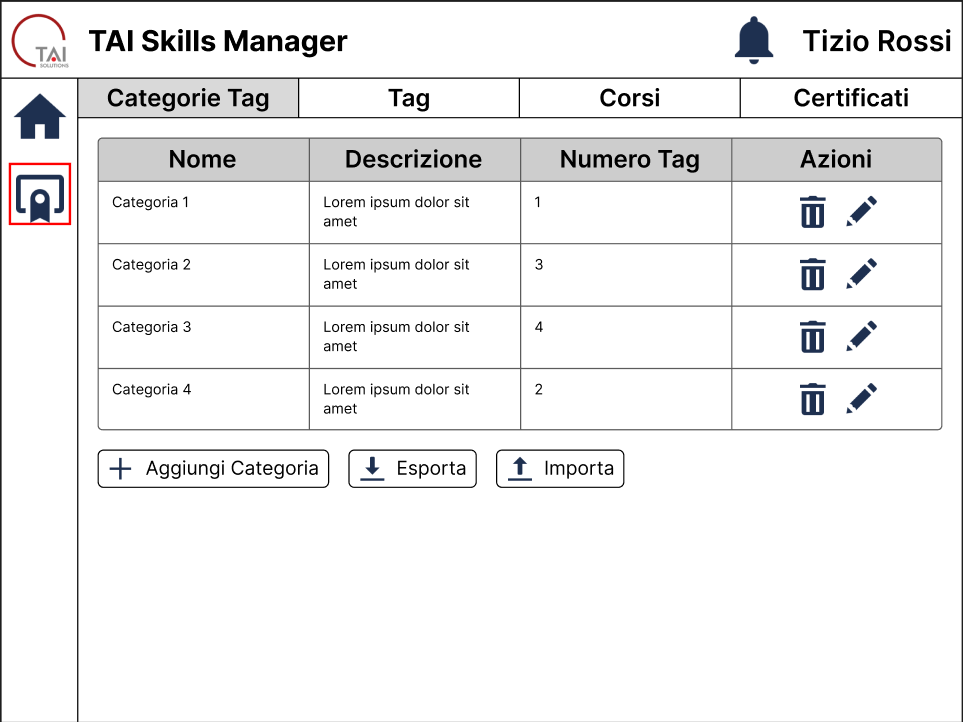
\includegraphics[width=0.7\linewidth]{immagini/mockup/Pagina Risorse Data Manager.png}
        \caption{Mockup della pagina Risorse di un Data Manager}
        \label{mockup-risorse}
\end{figure}
\FloatBarrier

\subsubsection{Skills User}
Nella pagina Skills Matrix, l’utente può cercare gli utenti per nome, o filtrare in base alle skill e categorie del sistema, per sapere chi possiede una specifica skill. Questo, ad esempio, può essere utile per sapere a chi fare alcune domande specifiche.

\begin{figure}[ht!]  
    \centering
        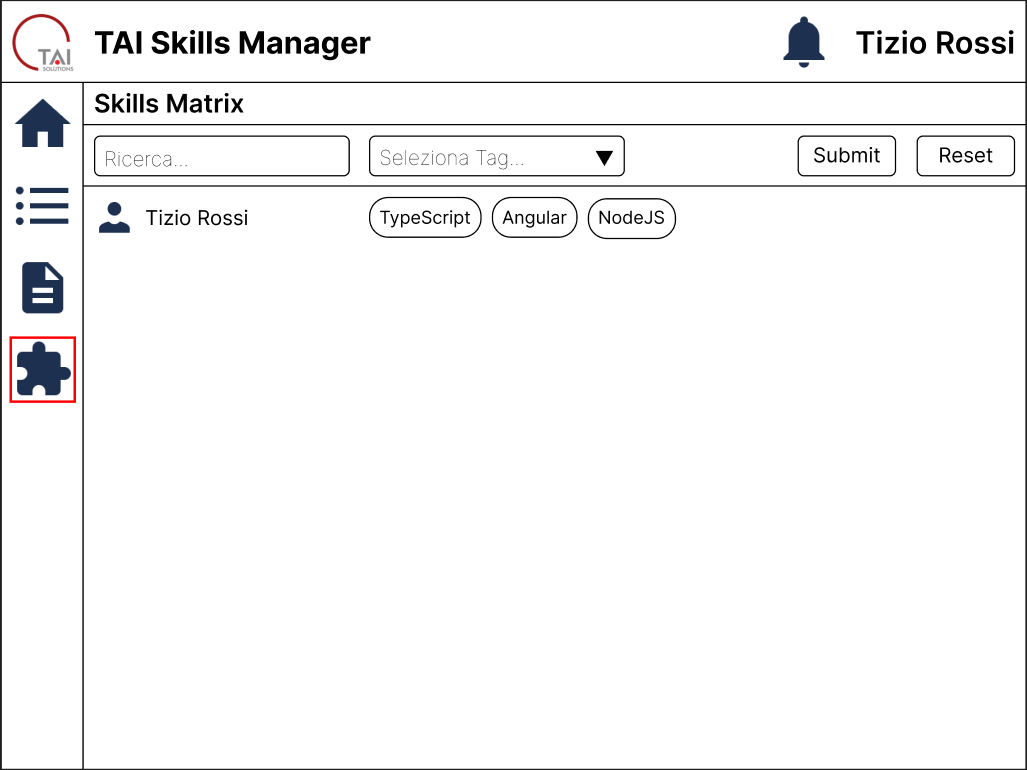
\includegraphics[width=0.7\linewidth]{immagini/mockup/Pagina Skills Matrix Skill User.png}
        \caption{Mockup della pagina Skills Matrix}
        \label{mockup-skills-matrix}
\end{figure}
\FloatBarrier

\subsubsection{Amministratore}
Dalla barra laterale sarà possibile accedere alla pagina Database, dove interagire con l’intero database per modifiche e esportazioni.

\begin{figure}[ht!]  
    \centering
        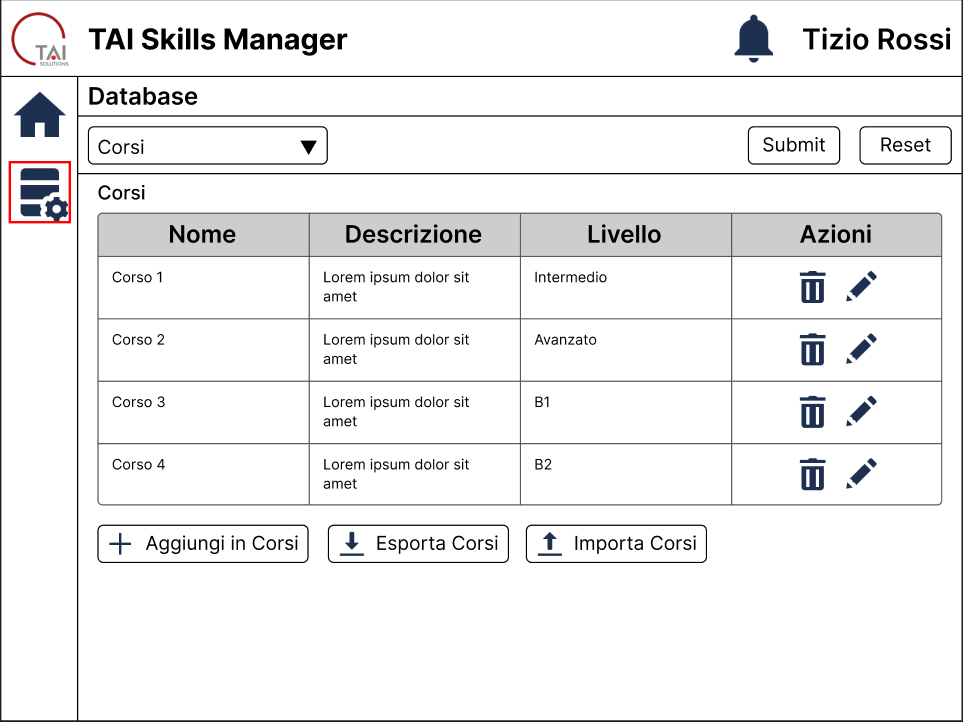
\includegraphics[width=0.7\linewidth]{immagini/mockup/Pagina Database Admin.png}
        \caption{Mockup della pagina Database di un Amministratore}
        \label{mockup-database}
\end{figure}
\FloatBarrier

\subsubsection{Notifiche}
Cliccando sull’icona della campanella in alto a destra, ciascun utente potrà visualizzare una sidebar a comparsa, contenente le sue notifiche.

\begin{figure}[ht!]  
    \centering
        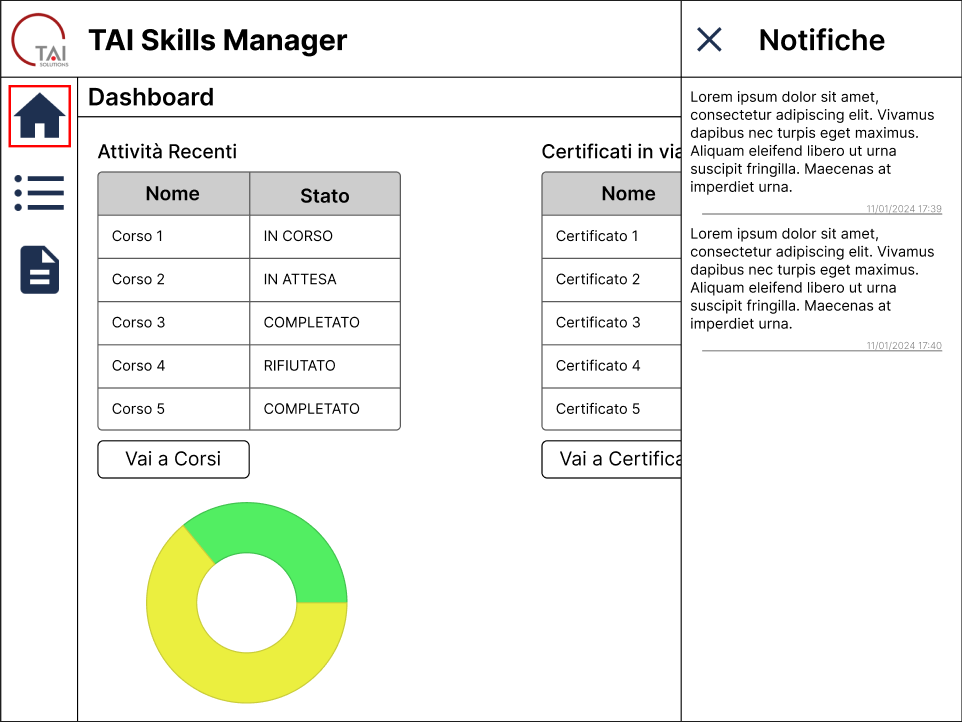
\includegraphics[width=0.7\linewidth]{immagini/mockup/Notifiche aperte su Dashboard Membro del Team.png}
        \caption{Mockup della Sidebar Notifiche}
        \label{mockup-notifiche}
\end{figure}
\FloatBarrier


\subsection{Accessibilità}
Considerato lo specifico contesto assolutamente ristretto in cui ci si trova ad operare e l’audience, non è richiesta la verifica di criteri di accessibilità.

\section{Specifiche non funzionali}

\subsection{Usabilità}
L’applicativo viene progettato per favorire l’utilizzo anche da parte di utenze meno esperte, pur mantenendo la completezza e la complessità richiesta dalle procedure implementate. Laddove possibile si rifarà uso di pattern grafici omogenei al fine di minimizzare il disorientamento dell’utente nell’utilizzo della GUI, facilitare l’apprendimento dei procedimenti e delle funzionalità del software, e creare un’esperienza di lavoro fluida e coerente.
\subsection{Sicurezza e accessi}
L’autenticazione degli utenti viene fatta mediante login con Google con il proprio account aziendale. La restrizione agli accessi degli utenti e le loro autorizzazioni utilizzano lo standard Role-Based-Access-Control (RBAC) attraverso il quale sono individuate le risorse/azioni a cui hanno accesso e il concetto di ruoli e permessi presenti nel sistema.
\subsection{Conformità normative}
Il sistema deve garantire la conformità ai requisiti delle normative ISO9001 e ISO27001.
\subsection{Scalabilità e Disponibilità}
Il sistema deve essere in grado di gestire un numero crescente di utenti e corsi nel tempo. Deve rispondere rapidamente durante l'accesso ai dati. 
\subsection{Integrazioni}
Il sistema deve essere predisposto per una futura integrazione con altri sistemi aziendali.
\subsection{Formati supportati}
Il sistema, per implementare la funzionalità dell’Amministratore di import ed export del database, inizialmente deve supportare il formato CSV, e rimanere compatibile con altri formati in una futura implementazione.

\section{Progettazione}

\subsection{Progettazione database}
Questa sezione illustra la modellazione del database per il sistema. La progettazione di un database efficace è fondamentale per garantire un'architettura solida e una gestione efficiente dei dati all'interno del sistema. Durante questa fase, sono stati sviluppati due diagrammi: uno concettuale e uno logico. Il diagramma concettuale rappresenta la struttura concettuale del database, definendo le entità, le relazioni e gli attributi dei dati. Il diagramma fisico, invece, trasforma il modello logico in uno schema dettagliato, specificando i tipi di dati, le chiavi primarie e esterne, nonché altre proprietà specifiche del database. Questi diagrammi forniscono una panoramica chiara della struttura del database e costituiscono la base per l'implementazione e la gestione dei dati all'interno del sistema.

\begin{figure}[ht]  
    \centering
    \makebox[\textwidth][c]{%
        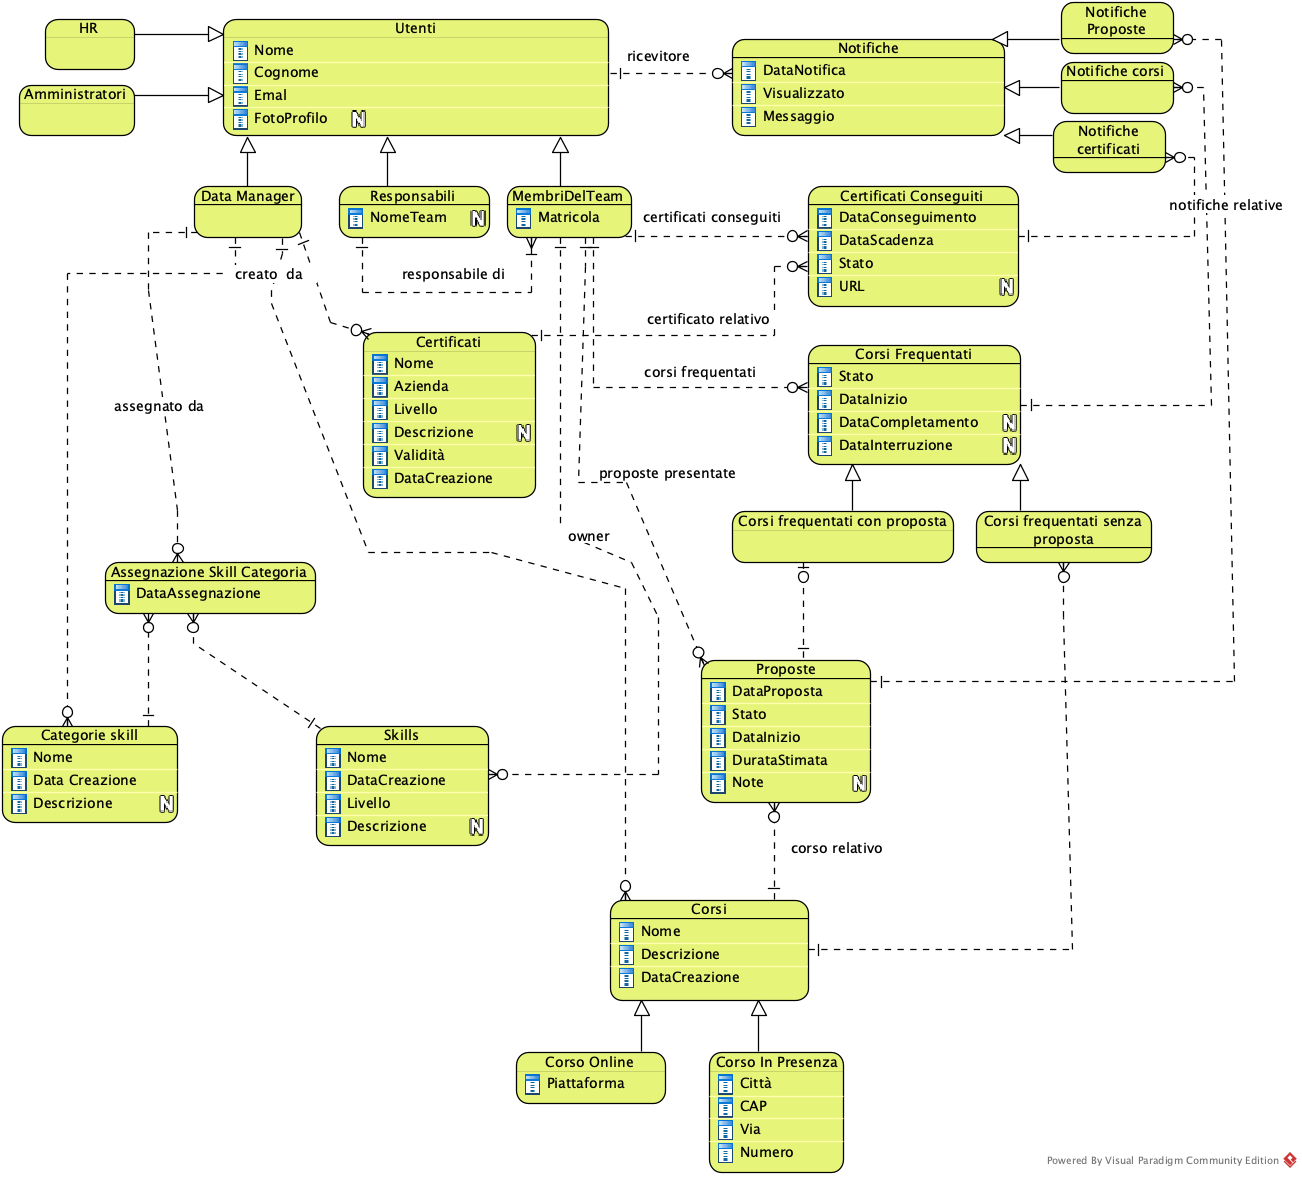
\includegraphics[width=1.1\linewidth]{immagini/db_concettuale.png}%
    }
    \caption{Diagramma E/R concettuale del database}
    \label{db_concettuale}
\end{figure}

\begin{figure}[ht]  
    \centering
    \makebox[\textwidth][c]{%
        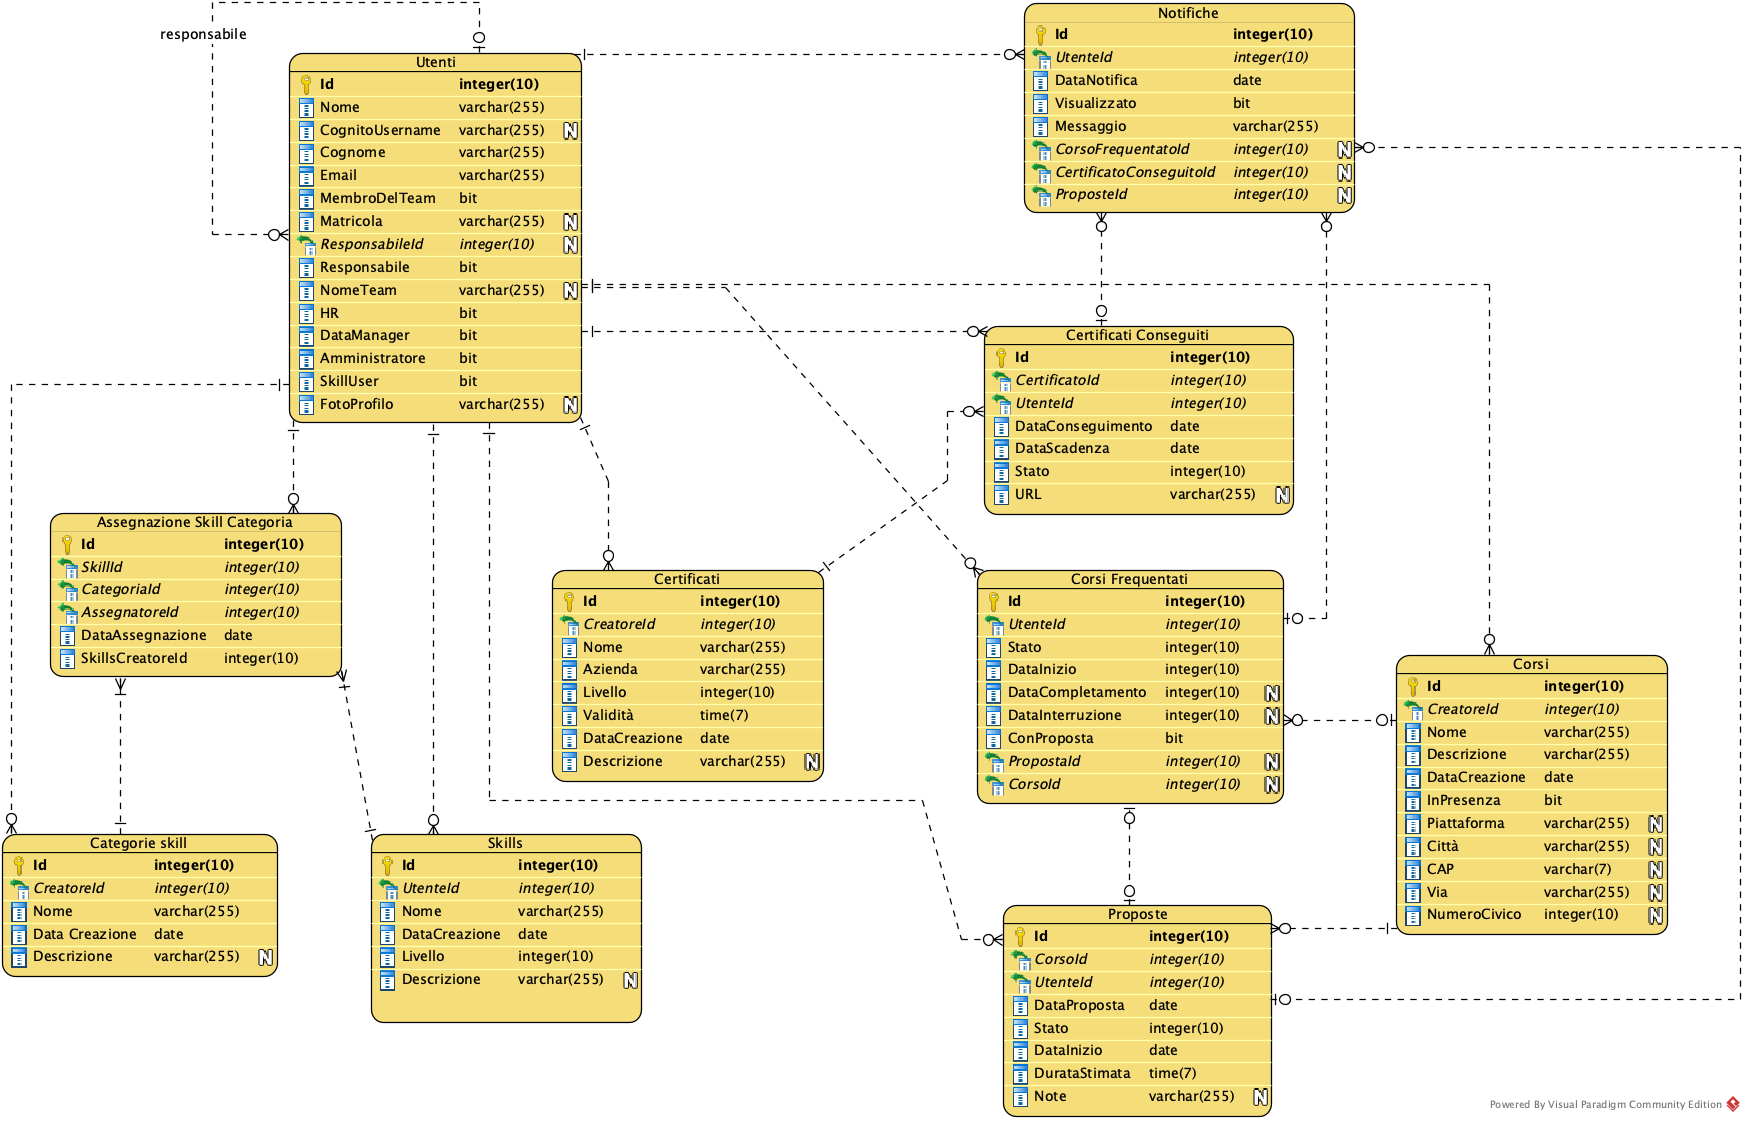
\includegraphics[width=1.1\linewidth]{immagini/db_logico.png}%
    }
    \caption{Diagramma E/R logico del database}
    \label{db_logico}
\end{figure}


\FloatBarrier

\subsubsection{Vincoli e dettagli non catturati graficamente}

Un corso frequentato può essere collegato ad una proposta, oppure direttamente ad un corso per quelli già completati o assegnati da un responsabile. Quindi non possono essere completati entrambi i cambi allo stesso momento.

\begin{itemize}
\item \textbf{CertificatiConseguiti.stato}: [conseguito, scaduto]
\item \textbf{Proposte.stato}: [inCreazione, inApprovazione, rifiutata, approvata]
\item \textbf{CorsiFrequentati.stato}: [iniziato, finito, nonCompletato]
\end{itemize}

La proprietà Livello di certificato e skill può essere tra 1, 2, 3.


\subsection{Progettazione API}
\label{openapi_spec}
Per la progettazione e la documentazione della REST API è stato adottato lo standard \texttt{OpenAPI 3.0} \cite{documentazioneOpenApi}. Questo approccio ha fornito un metodo strutturato per formalizzare i path dell servizio e specificare dettagliatamente i metodi HTTP supportati, i parametri richiesti e le risposte attese per ciascuna operazione.

Lo standard OpenAPI è una scelta eccellente per progettare e documentare le API, in quanto adotta un approccio "spec-first", dove la documentazione viene creata prima dell'implementazione effettiva. Utilizzare questo approccio consente di avere una visione chiara delle funzionalità dell'API e dei relativi requisiti, facilitando la progettazione e garantendo coerenza nell'implementazione.

La definizione dell'API funge da \texttt{"contratto"} tra il backend e il frontend. Durante la fase di progettazione, io e il mio collega ci siamo accordati sui vari formati di risposta e di richiesta per poi utilizzare questo file come principale punto di riferimento per l'implementazione.

È da notare che un file OpenAPI può essere scritto sia in formato JSON che YAML. Per questa specifica applicazione, è stato scelto il formato YAML in quanto rende la scrittura meno verbosa eliminando le parentesi degli oggetti JSON, rendendo il file più leggibile e manutenibile.

Infine, lo standard OpenAPI 3.0 si integra facilmente con generatori di codice e strumenti di documentazione come \href{https://swagger.io/}{Swagger}, consentendo di generare automaticamente la documentazione dell'API a partire dal file OpenAPI. Questo facilita notevolmente il processo di sviluppo, fornendo strumenti che supportano sia la fase di progettazione che quella di implementazione dell'API.

\subsubsection{Best Practices per il Design delle API REST}

Prima di procedere con la definizione dei path dell'API, è stata condotta un'attenta ricerca sulle best practices riguardanti le naming conventions e il design delle API REST. È stato fondamentale seguire standard e convenzioni ampiamente riconosciute per garantire coerenza, facilità di comprensione e interoperabilità tra me e il mio collega.

\subsubsection{Versione Iniziale e Aggiornamenti Successivi}

Il processo di creazione del file OpenAPI 3.0 è iniziato con la redazione della versione iniziale, che ha delineato i principali path e operazioni supportate dall'API. Durante questa fase, sono stati definiti i nomi dei path in base alle risorse e alle azioni che dovevano essere eseguite su di esse.

Successivamente, man mano che il sistema veniva implementato e nuove funzionalità venivano aggiunte o modificate, il file OpenAPI è stato aggiornato per riflettere le modifiche apportate. Questo approccio iterativo ha consentito di mantenere sempre aggiornata la documentazione dell'API e di garantire coerenza tra la progettazione e l'implementazione effettiva del sistema.

\vspace{0,3cm}

Di seguito un esempio di definizione di un percorso in una specifica YAML OpenApi per ottenere un certificato singolo conoscendo l'ID:

\lstinputlisting[
    language=yaml-openapi,
    caption={Esempio path OpenApi in YAML},
    label={lst:openapi}
]{code/api/openapi_getCertificate.yaml}

All'interno della definizione, sono stati inclusi i seguenti elementi:

\begin{itemize}
    \item \label{Tags}
    \texttt{Tags:} Utilizzati per l'organizzazione della documentazione, sono raggruppati sotto "Certificati" e sotto ai ruoli che possono fare quell'azione. Questo aiuta a categorizzare e identificare facilmente gli endpoint relativi ai certificati. Inoltre i tags relativi ai ruoli, definiscono chi può accedere alla risorsa e quindi fornire una visione chiara per l'implementazione (Admin è implicito in ogni percorso).
    \item \texttt{Summary:} Breve descrizione dell'obiettivo del percorso, che è ottenere un certificato singolo per ID. Fornisce una visione generale dell'azione che l'endpoint svolge.
    \item \texttt{OperationID:} Utilizzato per dare un identificatore univoco ad ogni endpoint. Questo aiuta a distinguere chiaramente gli endpoint e a facilitare il riferimento ad essi all'interno della specifica.
    \item \texttt{Description:} Descrizione dettagliata del percorso, che può includere informazioni su eventuali restrizioni o effetti a cascata sul sistema. Questo fornisce una spiegazione completa dell'endpoint e del suo utilizzo.
    \item \texttt{Parameters:} Includono i parametri attesi dall'endpoint, come ad esempio il "certificate\_id", che è specificato come un parametro di percorso usato per ottenere il certificato desiderato.
    \item \texttt{Responses:} Le possibili risposte che possono essere restituite dal percorso, tra cui il successo (codice '200'), la mancanza di un certificato (codice '404'), e errori del server (codice '500'). Questo fornisce un'indicazione delle diverse situazioni che l'utente potrebbe incontrare quando utilizza l'endpoint.
\end{itemize}

\subsubsection{Paginazione e Filtri}
\label{Paginazione}

Per gestire le chiamate che richiedono tutti gli elementi di una risorsa, abbiamo implementato la funzionalità di paginazione e previsto la possibilità di filtrare e ordinare per ogni campo di una risorsa.
Per la paginazione, abbiamo scelto di utilizzare il metodo limit-offset.
Per i filtri, abbiamo previsto diverse operazioni, sia unarie che binarie, nel formato nome:operazione{:valore} (con valore per le operazioni binarie), tra cui: contains, isNull, startsWith, equals e molte altre.
Per quanto riguarda l'ordinamento, abbiamo adottato il formato nome:[ASC|DISC].
Di seguito è riportata la definizione della chiamata GET /users, dove vengono specificati i parametri di paginazione, il valore di ritorno e gli eventuali errori che può ritornare.

\lstinputlisting[
    language=yaml-openapi,
    caption={Definizione OpenApi del path GET /users per ottenere tutti gli utenti del sistema},
    label={lst:openapi_getAll}
]{code/api/openapi_getAllUsers.yaml}

Da notare che filter e sort sono definiti come array, per permettere di applicare molteplici filtri e ordinamenti insieme. 
% multivaluequerystringparameters - no standard
% non cè scritto nella sezione  3.4 Query di RFC 3986

\vspace{0,3cm}

Per la visualizzazione dettagliata degli endpoint della REST API rimandiamo a Swagger Hub con la definizione OpenApi aggiornata:

\begin{itemize}
    \item \url{https://app.swaggerhub.com/apis/Lupetti-Lorenzo/SkillsManager/1.0.0#/}
\end{itemize}

Gli endpoint sono organizzati per risorse e per ruoli, per ruoli sono le chiamate che ogni ruolo può effettuare.
